\documentclass[12pt,pdf,hyperref={unicode}]{beamer}
%\usetheme{boxes}
\beamertemplatenavigationsymbolsempty
\setbeamertemplate{footline}[page number]
% Set it for the internal PhD thesis defence to reduce number of slides
%\setbeamersize{text margin left=0.5em, text margin right=0.5em}

\usepackage[utf8]{inputenc}
%\usepackage[english, russian]{babel}
\usepackage{bm}
\usepackage{multirow}
\usepackage{ragged2e}
\usepackage{indentfirst}
\usepackage{multicol}
\usepackage{subfig}
\usepackage{amsmath,amssymb}
\usepackage{enumerate}
\usepackage{mathtools}
\usepackage{comment}
\usepackage[all]{xy}
\usepackage{tikz}
\usetikzlibrary{positioning,arrows}
\tikzstyle{name} = [parameters]
\definecolor{name}{rgb}{0.5,0.5,0.5}

%\usepackage{caption}
%\captionsetup{skip=0pt,belowskip=0pt}

%\newtheorem{theorem}{Theorem}
%\newtheorem{statement}{Statement}
%\newtheorem{definition}{Definition}

% colors
\definecolor{darkgreen}{rgb}{0.0, 0.2, 0.13}
\definecolor{darkcyan}{rgb}{0.0, 0.55, 0.55}
%\AtBeginEnvironment{figure}{\setcounter{subfigure}{0}}
%\captionsetup[subfloat]{labelformat=empty}

%----------------------------------------------------------------------------------------------------------

\title{The Impact of Synthetic Data on Text Summarization Quality}
%\author{Name Surname}
%\institute[]{}
%\date{2024}

%---------------------------------------------------------------------------------------------------------
\begin{document}
%----------------------------------------------------------------------------------------------------------
\begin{frame}{The Impact of Synthetic Data on Text Summarization Quality}
    \begin{block}{Problem}
        Russian text summarization models face challenges due to a scarcity of high-quality, diverse labeled datasets, limiting their performance.
    \end{block}
    \vfill
    \begin{block}{Method}
        We will analyze the optimal ratio of synthetic to real data for diverse domains, assess the impact of semantic filtering, and evaluate model adaptation across architectures and domains.    \end{block}
    \vfill
    \begin{block}{Contribution}
        Design and implementation of synthetic data generation techniques and analysis of their impact on summarization quality.
    \end{block}
\end{frame}

\begin{frame}{Data Description}
    \textbf{Datasets:}
    \begin{itemize}
        \item Real data: \\ Gazeta, WikiLingua, Matreshka, DialogSum, etc. \\ $\approx$200k samples in Russian without long context, covering several domains.
        \item Synthetic data: \\ Automatically generated summaries to complement existing datasets. \\ \textbf{Expected Benefits:} Enhanced performance by eliminating domain gaps and enriching linguistic diversity, evaluated using both classical (e.g., ROUGE, BLEU) and advanced metrics (e.g., BERT Score).
    \end{itemize}
\end{frame}

\begin{frame}{Error Analysis and Expected Plots}
    \footnotesize
    \begin{columns}[T]
        \begin{column}{0.4\textwidth}
            \textbf{Analysis Plan:}
            \begin{itemize}
                \item \textbf{Impact of Synthetic Data and Semantic Filtering:}
                      Compare model metrics with varying proportions of synthetic data and evaluate the effect of semantic filtering.
                \item \textbf{Noise Impact:}
                      Assess models stability by adding noise to synthetic data.
                \item \textbf{Learning Curve:}
                      Track metrics changes over iterations with various data compositions.
            \end{itemize}
        \end{column}
        \begin{column}{0.6\textwidth}
            \vspace{1cm}
            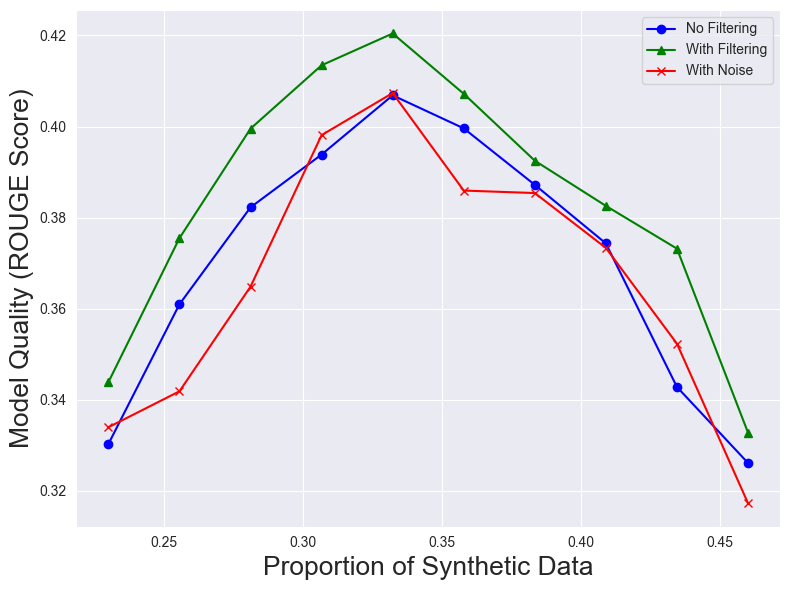
\includegraphics[width=\textwidth]{output.png}
            {\scriptsize The impact of synthetic data, noise, and filtering on quality.}

        \end{column}
    \end{columns}
\end{frame}


\end{document}